\documentclass[12pt,twoside]{article}
\usepackage[dvipsnames]{xcolor}
\usepackage{amsmath}
\usepackage{tikz,graphicx,amsmath,amsfonts,amscd,amssymb,bm,cite,epsfig,epsf,url}
\usepackage[hang,flushmargin]{footmisc}
\usepackage[colorlinks=true,urlcolor=blue,citecolor=blue]{hyperref}
\usepackage{amsthm,multirow,wasysym,appendix}
\usepackage{array,subcaption} 
% \usepackage[small,bf]{caption}
\usepackage{bbm}
\usepackage{pgfplots}
\usetikzlibrary{spy}
\usepgfplotslibrary{external}
\usepgfplotslibrary{fillbetween}
\usetikzlibrary{arrows,automata}
\usepackage{thmtools}
\usepackage{blkarray} 
\usepackage{textcomp}
\usepackage[left=0.8in,right=1.0in,top=1.0in,bottom=1.0in]{geometry}
\usepackage{pdfpages}
\title{1002 Midterm Cheat Sheet / Notes}
\author{USE AT YOUR OWN DISCRETION, THERE MIGHT BE TYPOS}
\date{October 2021}

\newcommand{\ra}{\Tilde{a}}
\newcommand{\rt}{\Tilde{t}}






\begin{document}

\maketitle

\newpage

\section{Probability}
\textbf{Conditional Probability:}
$$
    P(B|A) =\frac{P(A\cap B)}{P(A)}
$$  
\textbf{Chain rule (2 events):}
\begin{equation}
    \begin{split}
         P(A\cap B) &= P(A)P(B|A)  \\
                &= P(B)P(A|B)
    \end{split}
\end{equation}
\\
\textbf{DeMorgan's Law}\\

\textbf{More DeMorgan's Law}
\begin{equation}
    \begin{split}
        \text{One identity:} (A\cup B)^c &= A^c\cap B^c\\
        \text{Another Identity} (A\cap B)^c &= A^c \cup B^c
    \end{split}
\end{equation}

\textbf{For two events}
$$
    P(A\cup B) = P(A)+P(B) - P(A\cap B)
$$
\textbf{For three events}
$$
    P(A\cup B \cup C) = P(A)+P(B)+P(C) - P(A\cap B) - P(B\cap C) - P(A\cap C) + P(A\cap B \cap C)
$$

Chain rule (many events):
\begin{equation}
    \begin{split}
        P(A\cap B\cap C) &= P(A)P(B\cap C | A)\\
                            &= P(A)P(B|A)P(C|A\cap B)
    \end{split}
\end{equation}
Note the order of terms is arbitrary, can pull out B, or C first if we wanted. Consider what we know and choose wisely.\\

\textbf{Law of Total Probability:}
\begin{equation}
    \begin{split}
        P(B) &= \sum_{i}P(B\cap A_i)\\
        &= \sum_i P(A_i)P(B|A_i)
    \end{split}
\end{equation}
Where $A_1,\dots,A_n$ are disjoint events. \\

\textbf{Bayes Rule:}
\begin{equation}
    \begin{split}
        P(A|B) = \frac{P(A)P(B|A)}{P(B)}
    \end{split}
\end{equation}

\textbf{Independence of Two Events}
\begin{equation}
\begin{split}
    P(A|B) = P(A) \text{ and } P(A\cap B) = P(A)P(B)
\end{split}
\end{equation}
Only if the two events A,B are independent. \\

\textbf{Conditional Independence}
\begin{equation}
    \begin{split}
        P(A|B\cap C) = P(A|C) \text{ and } P(A\cap B|C) = P(A|C)P(B|C)
    \end{split}
\end{equation}


\section{Modeling Discrete Data}

\textbf{Popular distributions}
\begin{itemize}
    \item Binomial(n,p) = 
    $\begin{pmatrix}
    n \\
    k 
    \end{pmatrix} \times p^k \times (1-p)^{n-k}$
    \subitem Good for knowing the probability of K Coin flips being Heads out of N. N is the number of times you are flipping the coin, p is the chance of success (heads).
    \item Geometric(a) = $\alpha \times (1-\alpha)^{n-1}$
    \subitem Assumes that all events are independent, all probabilities are the same. With this formula, you are asking: whats the probability of getting a streak of heads that ends on the $a^{th}$ attempt? ($a-1$ heads, then 1 tails)
    \item Poisson Distribution: 
    $$P(\lambda) = \frac{\lambda^a \time e^{-\lambda}}{a!}$$
    \subitem that expresses the probability of a given number of events occurring in a fixed interval of time or space if these events occur with a known constant mean rate and independently of the time since the last event.
    \subitem a is the number of occurrences. IF you wanted to calculate $P(X>=3) = 1 - P(0) - P(1) - P(2)$
    \subitem As n approaches infinity, a binomial random variable with parameters, n and $\frac{\lambda}{n}$ tends to the distribution of a poisson distribution with parameter $\lambda$
    
    \subitem For any period of time of length $t$, if $t$ is small enough, the probability of an earthquake occurring in that period is equal to $\lambda$ and the probability of more than one earthquake is negligible. $\lambda$ is a fixed parameter representing the rate at which earthquakes occur.
    
    \subitem Each earthquake occurs independently from other earthquakes (we are ignoring aftershocks).
    \item \textbf{Negative Binomial} 
    $$
     \textbf{Negative Binomial } = \begin{pmatrix} k + r -1 \\ r\end{pmatrix} \times (1-p)^r \times p^k
    $$
    
    \subitem \textbf{Intuition} think of the dart problem on the homework.\\ 
\end{itemize}

\textbf{Combinatorics formula}  $$\frac{n!}{k!(n-k)!}$$
\newpage


\section{MLE For Discrete Distributions}
\begin{figure}[h!]
        \centering
        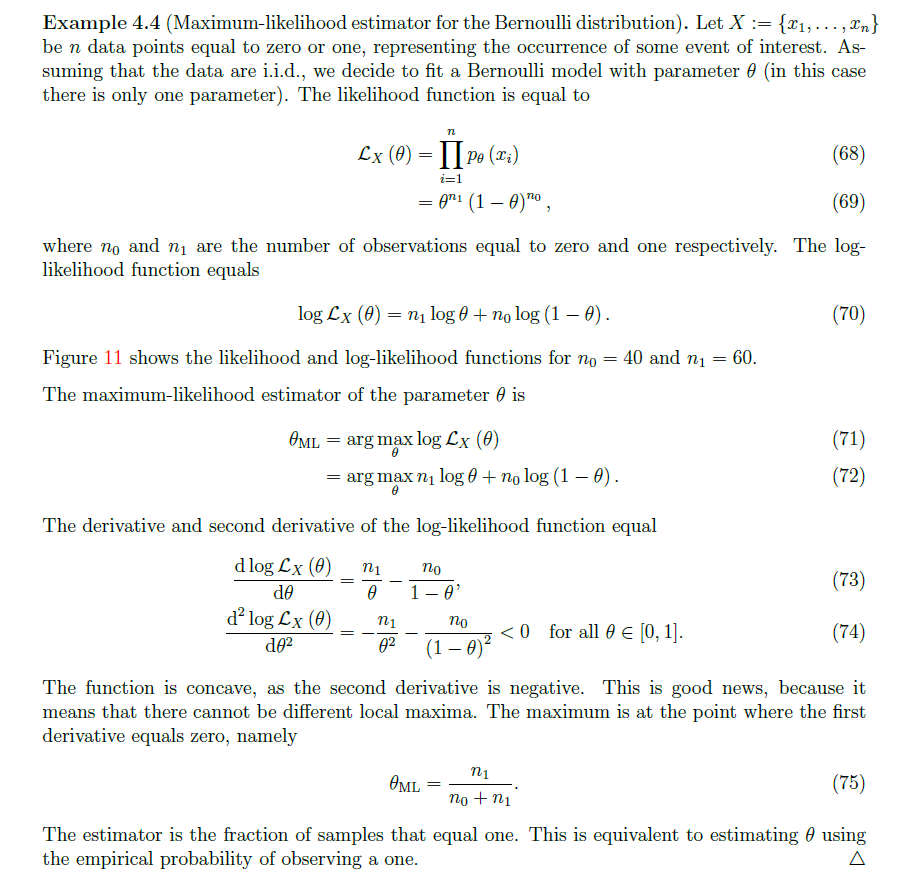
\includegraphics[scale=.75]{Pictures/loglikelihood_bernoulli.png}
        \caption{Bernoulli MLE}
        \label{fig:my_label}
    \end{figure}
    
\begin{figure}[h!]
        \centering
        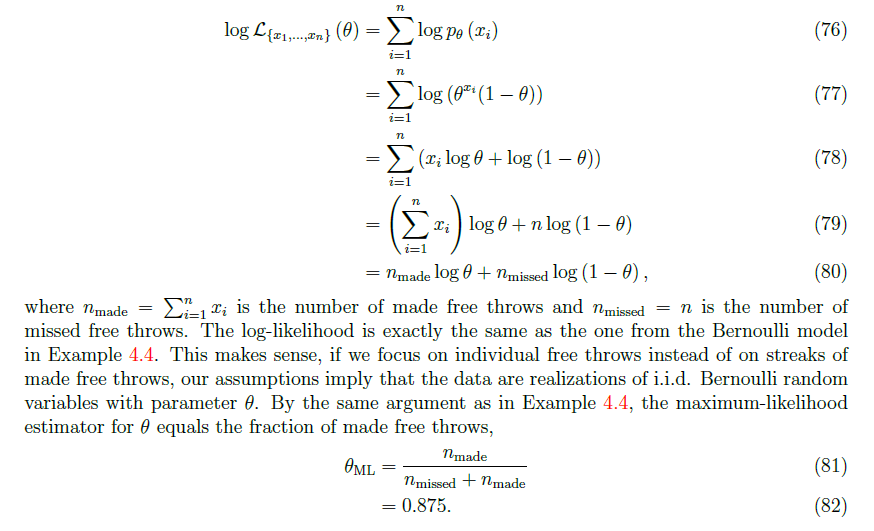
\includegraphics[scale=.6]{Pictures/loglikelihood_geometric.png}
        \caption{Geomtric MLE}
        \label{fig:my_label}
    \end{figure}


\begin{figure}[h!]
        \centering
        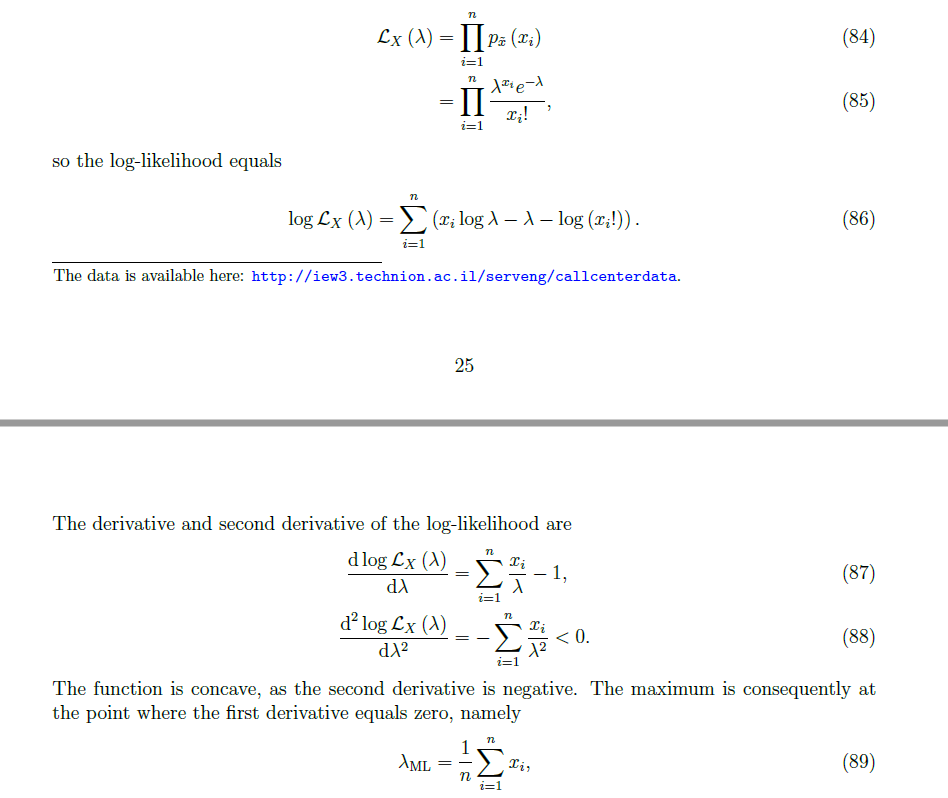
\includegraphics[scale=.5]{Pictures/loglikelihood_poisson.png}
        \caption{Poisson Discrete MLE}
        \label{fig:my_label}
    \end{figure}
\textbf{MLE for Gaussian Distribution}
Use mean and std dev of empirical data

\textbf{Uniform Distribution MLE}
a = min(data points), b = max(data points)
\newpage

\section{Modeling Continuous Data}

\textbf{Cumulative Distribution Funciton}
$$
    F_{\Tilde{a}}(a) = P(\Tilde{a}\leq a)
$$
The probability that $\Tilde{a} \leq a$. CDFs are always non-decreasing, and take values from [0,1].\\
Calculating a a probability of being in the the range of two values with cdfs:\\
\begin{equation}
    \begin{split}
         P(a<\Tilde{a}<b) &= F_{\Tilde{a}}(b) - F_{\Tilde{a}}(a)\\
         &= \int_a^b f_{\ra}(a)da
    \end{split}
\end{equation}
   


\textbf{Probability Density Function}\\
Captures the instantaneous rate of change of the random variable at that point, we obtain a PDF ($f_\ra$) by differentiating the CDF ($F_\ra$). Values in the PDF are not probabilities, but densities. You can have a value such that $f_{\ra} >1$. For a pdf to be valid, it must have only non negative numbers and integrate to 1.
$$
    f_{\ra}(a) = \frac{dF_{\ra}(a)}{da}
$$

\textbf{Kernel Density Estimate}
\begin{figure}[h!]
    \centering
    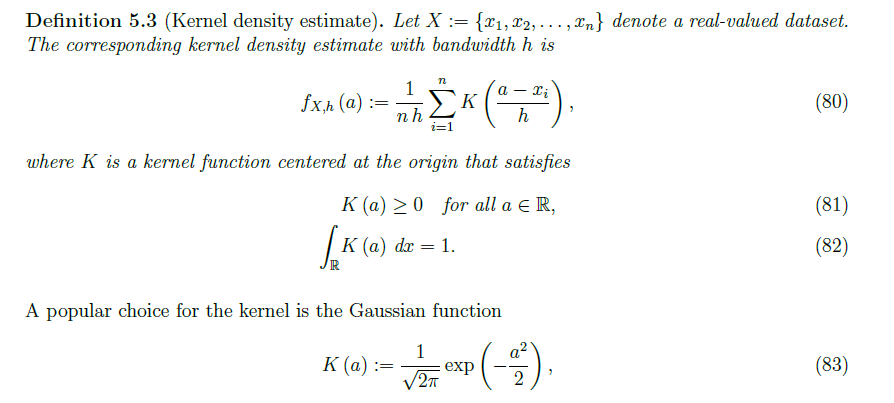
\includegraphics[scale=.7]{Pictures/KDE.png}
    \caption{KDE}
    \label{KDE}
\end{figure}
\begin{figure}
    \centering
    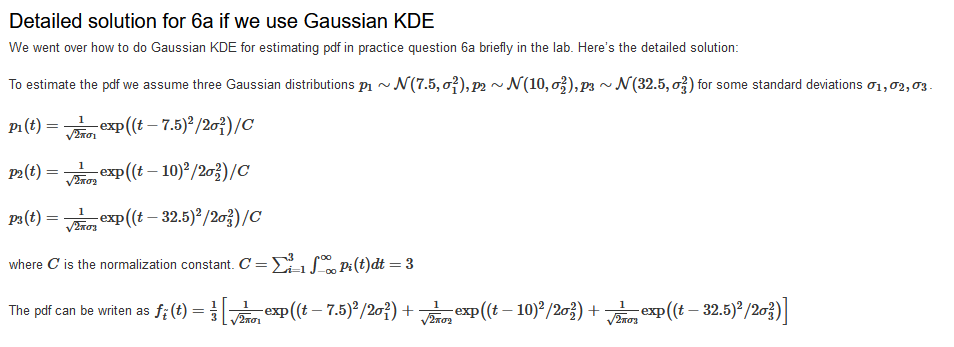
\includegraphics[scale=.7]{Pictures/kde gauss.png}
    \caption{KDE Example from Lab}
    \label{fig:my_label}
\end{figure}
\newpage

\section{Continuous Distributions}

\textbf{Continuous Uniform Distribution}\\
$$
    PDF = \frac{1}{b-a} \ \ \text{where a is the min range, b the max range of function}
$$
$$
    CDF = \begin{cases} 0 & for \  x<a \\ \frac{x-a}{b-a} & for \ x\in [a,b] \\ 1 & for \ x > b \end{cases}
$$
\textbf{Think of the uniform CDF as a straight line that connects 0 to 1 from a to b} \\

\textbf{Exponential Distribution PDF}\\
An exponential random variable $\rt$ with parameter $\lambda$ has a PDF:
$$
    PDF = f_{\rt}(t) = \begin{cases} \lambda e ^{-\lambda t}, & if \ t \geq 0, \\
    0, & otherwise.\end{cases}
$$
The exponential distribution is memoryless, such that when conditioning on a certain time $\rt|\rt>t_0$ we simply move over the exponential distribution $t-t_0$:
$$
    f_{\rt|\rt>t_0}(t) = \lambda e^{-\lambda (t-t_0)}
$$
\textbf{Exponential Distribution CDF}\\
$$
    CDF = F_{\rt}(t) = \begin{cases} 1 - e ^{-\lambda t}, & if \ t \geq 0, \\
    0, & otherwise.\end{cases}
$$
\textbf{Note if there's a scalar it gets preserved during integration. For example:}
$$
        PDF = \alpha \lambda e^{-\lambda t} \rightarrow CDF = F_{\rt}(t) = \begin{cases} 1 - \alpha e ^{-\lambda t}, & if \ t \geq 0, \\
    0, & otherwise.\end{cases}
$$
\textbf{Conditional CDF}
$$
    Conditional \ CDF = F_{\rt|\rt>t_0}(t) = 1 - e^{-\lambda(t-t_0)}
$$

\textbf{Gaussian Distribution}\\
Gaussian PDF with mean $\mu$ and variance $\sigma^2$ (N($mu$,$\sigma^2$)):
$$
    PDF = f_{\ra}(a) = \frac{1}{\sqrt{2\pi}\sigma}e^{-\frac{(a-\mu)^2}{2\sigma^2}}
$$

\textbf{MLE for Exponential}\\
\begin{figure}[h]
    \centering
    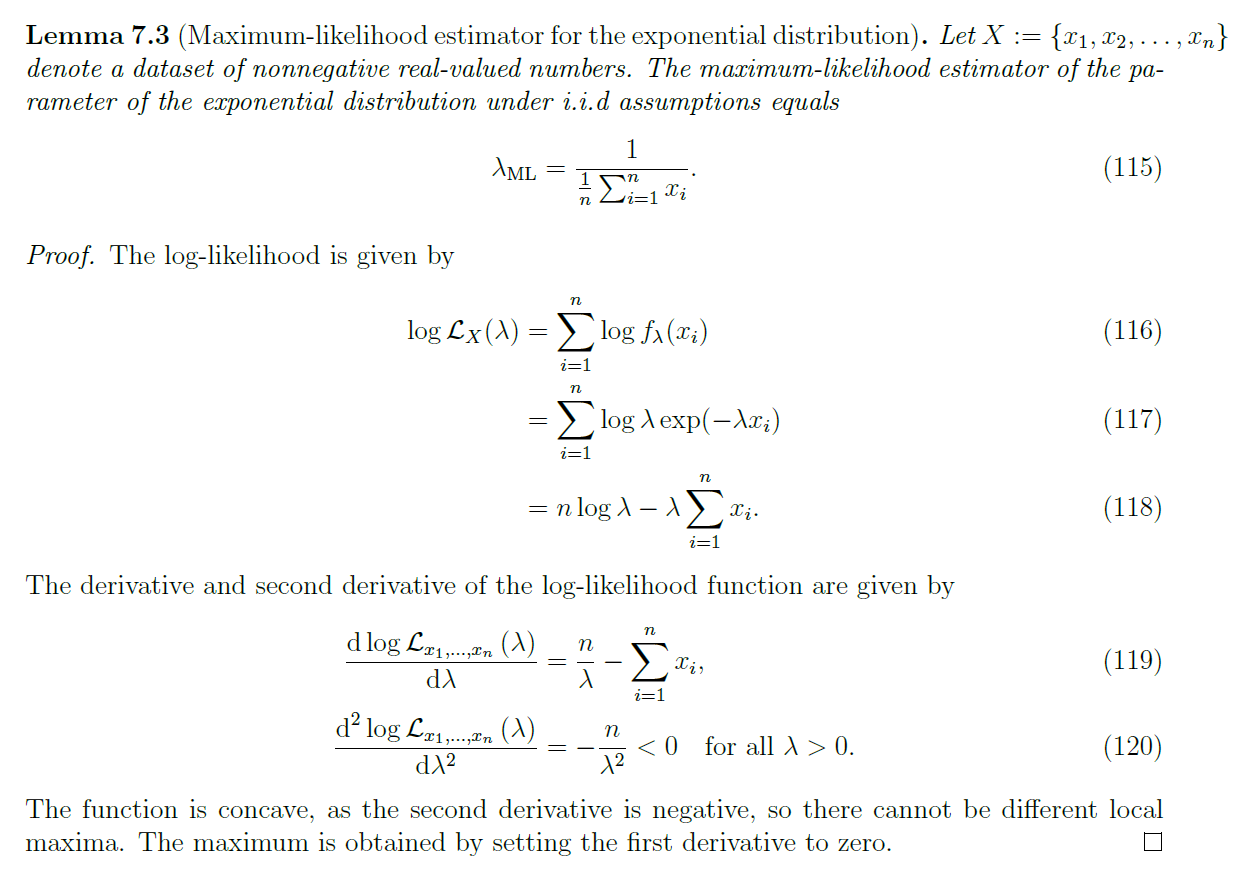
\includegraphics[scale=.38]{loglikelihood_exponential.png}
    \label{fig:my_label}
\end{figure}


\break

\textbf{Inverse Transform Sampling}\\
Two reasons: 
\begin{enumerate}
    \item Generating uniform samples from the unit interval [0,1]
    \item Transforming the uniform samples so they have the desired distribution
\end{enumerate}
    
\begin{figure}[h!]
    \centering
    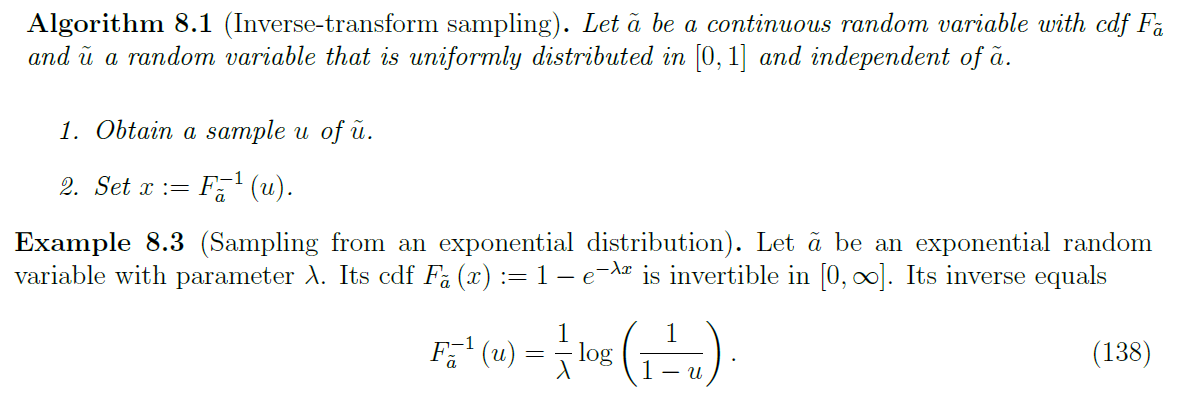
\includegraphics[scale=.5]{inverse-transform-sampling-exponential.png}
    \caption{Inverse Transform Sampling}
    \label{fig:my_label}
\end{figure}
\textbf{ Inverse Transform Sampling Algorithm:} when calculating the inverse cdf, integrate from the bottom range of each pdf to a random variable $\Tilde{t}$. Make sure, that if you have multiple pdfs (and are calculating multiple cdfs), you add the cumulative value after integrating. For example, if i have two pdfs, and the first cdf covers one half of the probability, then after integrating the second pmf to find the second cdf, add the value of 1/2 to the result. Then you can inverse by switching y,t to calculate inverse. Then plug in your sample according to the sample value (if I have a sample value $<$ 1/2 I would use the first cdf, if its greater I would use the second one). \\

\textbf{Intuition}: You have two use cases for inverse transform sampling:
\begin{itemize}
    \item You plug in a sample from a uniform distribution into a inverse cdf to get the corresponding pdf/cdf value that corresponds to the percentile of the sample from the uniform. I.e. You want to find the score you would need to be in the 90th percentile. You plug in .9 to the inverse cdf and you get the score you would need.
    \item The inverse is true. You can plug a pmf value into the inverse cdf to find the according percentile (uniform distribution sample).
\end{itemize}

\newpage 

\section{Modeling Multivariate Discrete Data}
\textbf{Joint PDFs}
Notation:
$$
    P_{\Tilde{a},\Tilde{b}}(a,b) = P(\Tilde{a}=a, \Tilde{b}=b) \qquad a \in R_{\Tilde{a}} \ \  b \in R_{\Tilde{b}}
$$
Joint pdfs must be non-negative (they represent probabilities), and must sum to 1.
$$
    \sum_{a\in R_{\Tilde{a}}} \sum_{b \in R_{\Tilde{b}}} p_{\Tilde{a},\Tilde{b}}(a,b) = 1
$$  
\textbf{Marginal PMF}
$$
    p_{\Tilde{a}}(a) = \sum_{b \in B} p_{\Tilde{a},\Tilde{b}}(a,b)
$$
\textbf{Naive Bayes}\\

Here we are trying to predict a classifier $y$ given some data that has features $x_1,x_2,\dots$. To keep things simple, in the formula below were assuming $y$ is a binary class (i.e. 1 is republican 0 is democrat) and we only have 3 features $x_1, x_2,x_3$
$$
    Naive \ Bayes = P(y|x_1\cap x_2 \cap x_3) = \frac{P(y\cap x_1 \cap x_2 \cap x_3)}{P(x_1\cap x_2 \cap x_3)} = \frac{P(y)P(x_1|y)P(x_2|y)P(x_3|y)}{\sum_{y=0}^1 P(y\cap x_1 \cap x_2 \cap x_3)}
$$
$$
    = \frac{P(y=1)P(x_1|y=1)P(x_2|y=1)P(x_3|y=1)}{P(y=1)P(x_1 |y=1)P(x_2|y=1)P(x_3|y=1) + P(y=0)P(x_1|y=0)P(x_2|y=0)P(x_3|y=0)}
$$
The features $x_1,x_2, x_3$ should all be set to some value as well, I just didn't have the space to do such notation.
\\

\textbf{Miscellaneous, (Geometric Series, Derivatives and Integrals)}\\

\textbf{Geometric Series}
\begin{equation}
\begin{split}
    \sum_{i=1}^{k} r^i &= \frac{r(1-r^i)}{1-r}
\end{split}
\end{equation}

\textbf{Note if r is a fraction, as k approaches infinity $r^i=0$ thus the top half of the equation will be just $r(1-0)=r$}

\begin{figure}[h!]    
\centering
    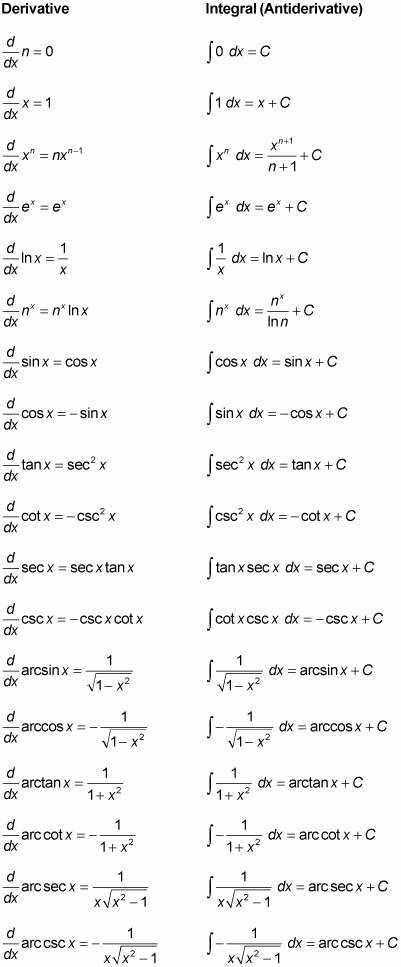
\includegraphics[scale=.7]{Pictures/diff and integration.png}
    \caption{Common Derivative and Integral Formula}
    \label{fig:my_label}
\end{figure}



\begin{figure}[h!]
    \centering
    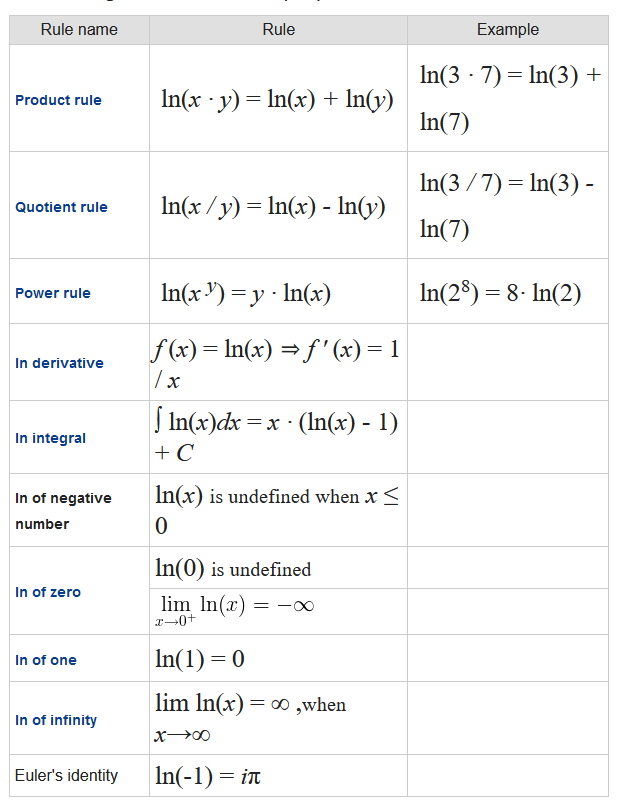
\includegraphics[scale=.8]{ln_properties.png}
    \caption{Properties of Natural Logarithm}
    \label{Ln properties}
\end{figure}
\end{document}
